\documentclass{bmvc2k}

%% Enter your paper number here for the review copy
%\bmvcreviewcopy{??}

\title{Object-Centric Spatio-Temporal Pyramids for Egocentric Activity Recognition}

% Enter the paper's authors in order
% \addauthor{Name}{email/homepage}{INSTITUTION_CODE}
\addauthor{Tomas McCandless}{tomas@cs.utexas.edu}{1}
\addauthor{Kristen Grauman}{grauman@cs.utexas.edu}{1}

% Enter the institutions
% \addinstitution{Name\\Address}
\addinstitution{
 Department of Computer Science \\ 
 University of Texas at Austin
}

\runninghead{McCandless, Grauman}{Object-Centric Spatio-Temporal Pyramids}

% Any macro definitions you would like to include
% These are not defined in the style file, because they don't begin
% with \bmva, so they might conflict with the user's own macros.
% The \bmvaOneDot macro adds a full stop unless there is one in the
% text already.
\def\eg{\emph{e.g}\bmvaOneDot}
\def\Eg{\emph{E.g}\bmvaOneDot}
\def\etal{\emph{et al}\bmvaOneDot}

%------------------------------------------------------------------------- 
% Document starts here
\begin{document}

\maketitle

\begin{abstract}
	Egocentric video and wearable computing have become increasingly
	prevalent in the past decade, resulting in a huge explosion in the amount
	of available video content and increased attention from the computer
  vision community.
  However, existing methods for activity recognition often use
  predefined spatio-temporal binning schemes
  to aggregate features. This encodes information beyond what is possible
  with a pure ``bag of words'' model, but is ultimately inflexible
  and may fail to capture important spatio-temporal relationships between
  features.
  We propose to randomly generate a pool of candidate binning schemes and
  use a boosting algorithm to combine those which are most discriminative. 
  In order to efficiently focus the candidate partition schemes, we
  create biased partitions using ``object-centric'' cuts in video volumes.
  Partition schemes generated using our method have a high probability of
  cutting through video regions that contain ``active objects,'' the objects
  being interacted with by the user during a given frame.
  Given a set of training videos, our method first computes histograms of
  active object locations across each $(x, y, t)$ dimension, then uses these
  histograms to generate a pool of object-centric partition schemes that
  have a high probability of cutting through regions that often contain
  active objects.
	We use a boosting algorithm to learn which partitioning schemes are
  most discriminative and form a
	final strong classifier. Our main novel contribution is two-fold: we show how to learn the
  most useful partition schemes in an egocentric setting, and we focus
  candidate partition schemes by exploiting locations of active objects.
  Our approach yields state-of-the-art recognition performance, and we find
  that object-centric partition schemes are often more discriminative than
  their unbiased counterparts.
\end{abstract}

%------------------------------------------------------------------------- 
\section{Introduction}
  % uses for egocentric activity
  % recent research without detailed explanation
	Activity recognition is becoming an increasingly canonical problem in
	computer vision as researchers are beginning to explore the domain more
  thoroughly and several relevant datasets have been released 
  \cite{Schuldt04, Rodriguez08, Fathi11, Ramanan12}. 
  Egocentric activity recognition differs from
  non-egocentric activity recognition because activities can have long-term
  temporal dependencies and actions can be interrupted by other actions. 
	% application to life logging
	A robust and accurate method for egocentric activity recognition would have 
	useful practical applications, such as a memory aid, content-based
  summarization, or telerehabilitation. For instance,
	a recent trend in wearable computing is so-called life logging which can
	assist patients suffering from memory loss \cite{Sellen07}. 
	A robust egocentric activity recognition
	system could automatically tag video clips with their corresponding types of activities.
  Additionally, there are many clinical benchmarks used to evaluate patients everyday
  functional abilities \cite{Kopp97, Catz97, Itzkovich07}. 
  These benchmarks are currently conducted in a
  hospital setting, but a robust system for egocentric activity
  recognition
  could greatly impact the workflow for patient evaluation, allowing
  for passive long term observation of patients in their own
  homes.
  Existing work has made promising progress in both recognition and
  summarization, \cite{Ramanan12, Fathi12,Lee12} 
  yet it remains a challenging problem.






  % egocentric defined by objects, binning with preservation of object
  % relationships is unclear.
  % existing work uses hand coding
  % cite ramanan, choi, laptev but not in detail
  Egocentric activities
  are well-defined by the types of objects that are interacted with by users
  during particular actions (``active objects'') \cite{Ramanan12}, yet how to optimally aggregate
  features across space-time remains unclear.
  The familiar bag-of-words approach can be used to aggregate 
  features with reasonable performance, but ultimately falls short because it
  fails to capture temporal dependencies between features.
  The pyramid is a well-known extension of a pure bag-of-words model that encodes spatial
  relationships between features by recursively subdividing images or video and extracting 
  features from each spatial bin \cite{Lazebnik06}, yielding impressive
  results across a range of applications.
  Existing methods for activity recognition often rely on
  hand-coded partition schemes \cite{Ramanan12, Choi08, Laptev08}.
  With a small pool of hand-coded schemes for imposing spatial
  information, the most discriminative space-time relationships between features may not be 
  captured. 
% it is problematic to use hand-coded partitions because...







  % our idea: learn partitions
  Our idea is to randomly generate a pool
  of candidate partitioning schemes. 
  We then aggregate spatio-temporal features in a
  learned way, using a boosting algorithm to select those partitioning schemes which are most discriminative.
  % focus the partition generation
  Boosting is computationally expensive in terms of the number of weak
  classifiers that are used, and there are many high-dimensional
  partitioning schemes we could sample. This suggests that a large pool of
  candidate partition schemes is required to obtain good performance.
  In order to avoid generation of partitions that are not discriminative, we
  introduce object-centric partitioning schemes, which have a high
  probability of cutting through video regions known to contain active
  objects.
  





  % method overview short, mention partition generation and boosting
  Given a set of labeled training videos with object annotations (bounding boxes and
  active/passive tags), our method first computes histograms of active
  object locations across each $(x,y,t)$ dimension of video. We use these
  histograms to generate a pool of object-centric partition schemes that have a high
  probability of cutting through regions known to frequently contain active
  objects. We compute feature vector representations of each training video clip using each
  candidate in the pool, and use these vectors to train a pool of weak SVM
  classifiers. Finally, we use a boosting algorithm to select the partitions
  which are most discriminative and form a final strong classifier.






  % results teaser -- not just improvement on stoa, but detail on what will
  % be shown
  We find that object-centric partitioning schemes that have a larger number
  of levels are often the most discriminative in the sense that they tend to
  get selected by boosting over their unbiased counterparts.
  We evaluate the performance of our method using a cross-validation
  experiment and find that our method using object-centric pyramids improves
  upon the current state of the art.





	

%-------------------------------------------------------------------------
\subsection{Related Work}

  %--------
  % activity recognition in general
  Activities in a non-egocentric setting can be effectively analyzed based
  on tracked limb shapes and motion across a video clip as in 
  \cite{Ramanan03, Rao01, Rodriguez08}. An
  alternative approach involves using lower-level features with weaker
  semantics such as space-time interest points as in \cite{Schuldt04,
  Laptev08}.
  Previous work on spatial pyramids \cite{Bosch07, Lazebnik06} is
  extended in \cite{Laptev08}
  by defining the spatio-temporal pyramid representation of video clips, but
  a relatively small number of predefined schemes for spatio-temporal
  binning are used,
  which may fail to capture important spatio-temporal relationships between
  features. There are 6 possible spatial grids and 4 temporal binning
  schemes, resulting in a total of 24 possible spatio-temporal partition
  schemes.
  % BoW methods for video (laptev, choi, ramanan)
  Bag of words as a method for pooling of space-time features in video has been
  analyzed in \cite{Choi08, Laptev08, Ramanan12,Marszalek09, Fathi11_}.




  % egocentric analysis: recognition, summarization.
  % yong jae, lu zheng, fathi/ren (and some of their refs)
  % main point: importance of objects in egocentric vs other cues in other
  % domains
  Egocentric video is an increasingly popular topic in the computer vision
  community. Recent work has explored discovery of important people for
  automatic summarization of egocentric
  video \cite{Lee12}. The relationship between gaze and activity in an
  egocentric setting is explored in \cite{Fathi12}, which presents methods
  to predict activity given gaze, gaze given activity, and both activity and
  gaze given neither. Object recognition in an egocentric setting has been
  explored with promising results by \cite{Ramanan12, Fathi11, Ren09}.
  Activity recognition in an egocentric context has been investigated by
  \cite{Ramanan12, Fathi11_}.
  The main work related to our own is that carried out in \cite{Ramanan12}, 
  which introduces the ADL dataset we use to benchmark our method, 
  as well as detailed analysis of the the
	performance of several different classifiers. 
	
  Existing work has established that egocentric activities are object-driven
  in the sense that visible objects provide useful cues about what types of
  activities are occurring, rather than tracking of limb position or
  summarization of overall motion. In other words,
	egocentric activity recognition is ``all about
  the objects'' \cite{Ramanan12}, particularly the objects being interacted
  with (``active objects''), as
	recognition accuracy increases dramatically when locations of active
  objects in addition to passive objects are used as features. 




  % spatial binning strategies
  % kovashka, lazebnik, sharma, jiang (but not too much credit to jiang)
  Selection of binning strategies for features in a learned way has been throrougly explored in the
  spatial domain \cite{Sharma11, Jiang12} for image recognition, and some
  analysis of learning shapes of spatio-temporal regions on a per-class
  basis using low-level features has been conducted in the video domain \cite{Kovashka10}, but to
  our knowledge selection of binning strategies in a learned way has not
  been explored specifically in the egocentric domain.
  
	
  
	We use a version of the SAMME multi-class Ada-boost algorithm \cite{Zhu06}
  with randomized spatio-temporal pyramids to explore discriminative
  selection of partitions for video data, specifically in the egocentric
  domain.

\section{Approach}
  The goal of our algorithm is to robustly predict what type of activity is occurring in
  an egocentric video clip. In contrast to other forms of action
  recognition, egocentric action is ``object-driven'' in the sense that
  activities are well-defined by the objects the user is interacting with in
  a particular video sequence. Figure 1 depicts example frames extracted from
  video sequences that show the visual differences between passive and
  active versions of the same objects.
  
  Existing methods for non-egocentric activity
  recognition often use space-time interest points \cite{Laptev03} as features. In other
  words, in a non-egocentric setting action recognition is often driven by
  summarization of motion cues throughout video, while object locations can
  serve as effective features in an egocentric setting.

  Active objects, those which are being interacted with by the user in a
  given video clip, are especially helpful features for egocentric activity
  recognition \cite{Ramanan12}, yet there is little work in the literature
  exploring the best ways to pool video features across space-time. A common
  technique for pooling features is ``bag-of-words'', an orderless histogram
  of feature counts. This technique is simple, but does not encode any
  potentially useful relationships between features in space-time. The
  ``pyramid'' is an extension to bag-of-words that encodes space-time
  relationships between features by recursively
  subdividing an image or video into multiple subregions and concatenating
  bag-of-words histograms computed for each region. 

\begin{figure}
  \begin{center}
\begin{tabular}{cc}
\bmvaHangBox{\fbox{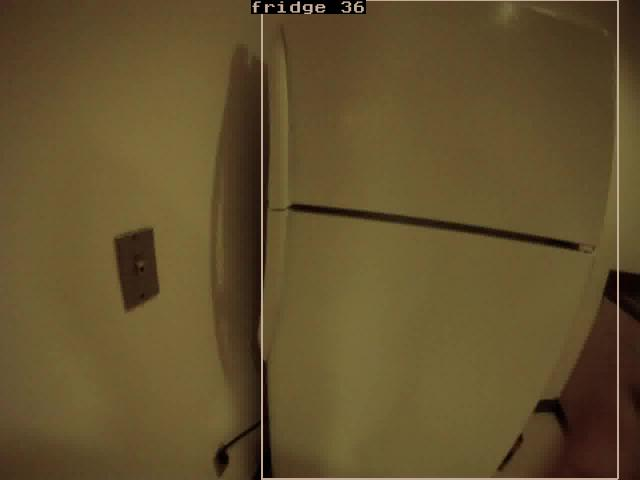
\includegraphics[width=4.0cm]{figures/activevpassive/fridge_passive.jpg}}}&
\bmvaHangBox{\fbox{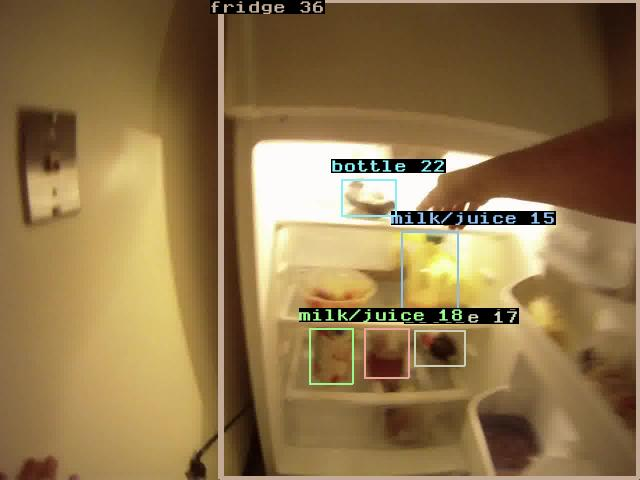
\includegraphics[width=4.0cm]{figures/activevpassive/fridge_active.jpg}}}\\
\bmvaHangBox{\fbox{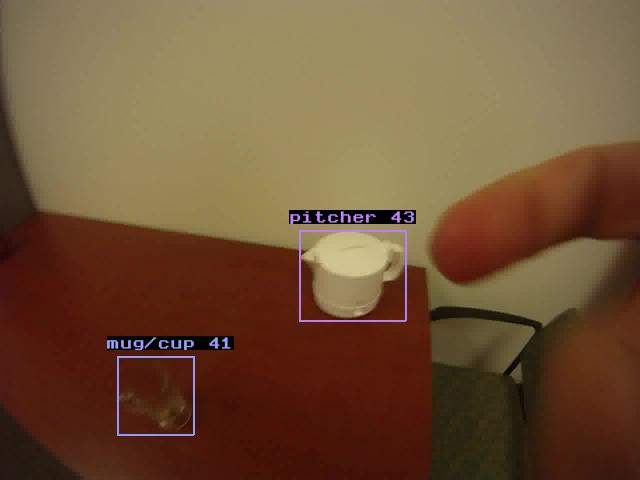
\includegraphics[width=4.0cm]{figures/activevpassive/mug_passive.jpg}}}&
\bmvaHangBox{\fbox{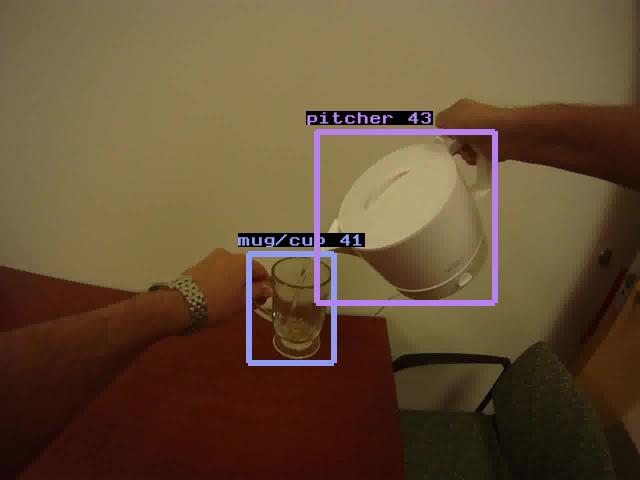
\includegraphics[width=4.0cm]{figures/activevpassive/mug_active.jpg}}}\\
\bmvaHangBox{\fbox{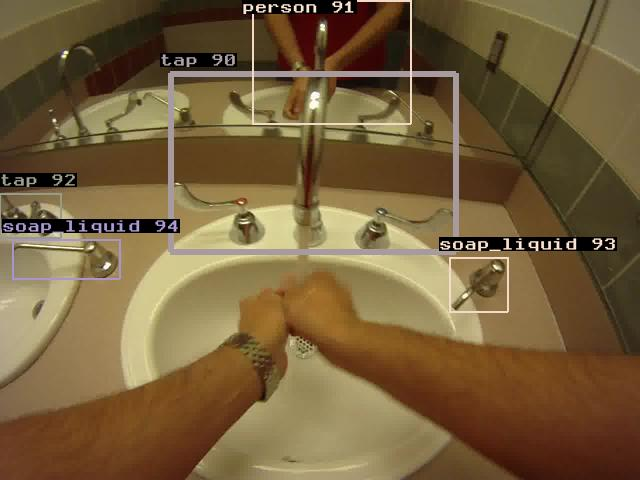
\includegraphics[width=4.0cm]{figures/activevpassive/soap_passive.jpg}}}&
\bmvaHangBox{\fbox{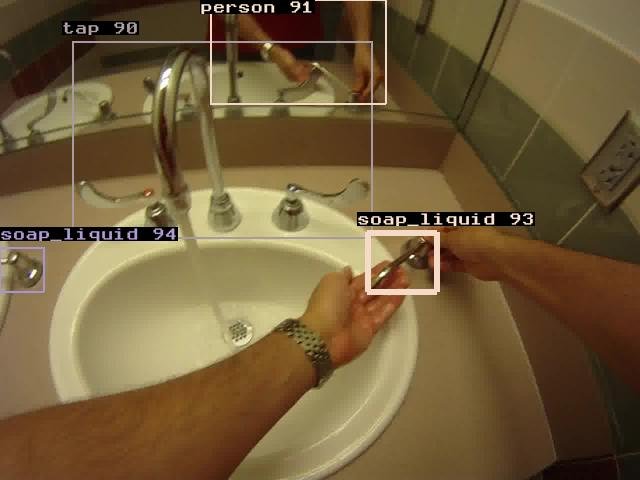
\includegraphics[width=4.0cm]{figures/activevpassive/soap_active.jpg}}}\\
\bmvaHangBox{\fbox{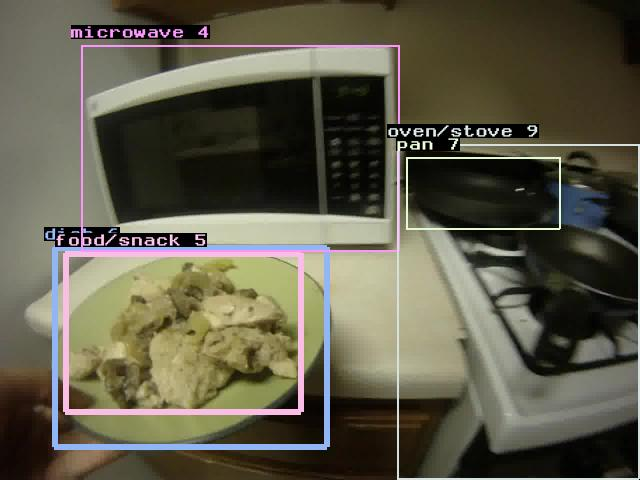
\includegraphics[width=4.0cm]{figures/activevpassive/micro_passive.jpg}}}&
\bmvaHangBox{\fbox{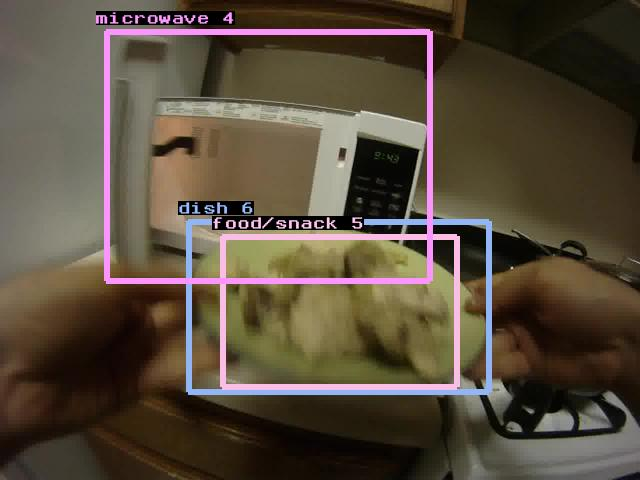
\includegraphics[width=4.0cm]{figures/activevpassive/micro_active.jpg}}}\\
\end{tabular}
		   \caption{Example frames extracted from the dataset. The left and
       right columns depict passive and active versions of the same objects,
     respectively.}
\label{fig:teaser}
  \end{center}
 \end{figure}
  Existing work relies on hand-coded partition schemes for computing
  pyramid representations of datapoints, which is a problematic approach
  because it is inflexible with respect to new data and can fail to capture
  the most meaningful relationships between features. To address this
  problem, we propose to randomly generate a pool of candidate partitioning
  schemes, then use a multi-class boosting algorithm to learn the most
  discriminative partition schemes and combine them into a final ``strong''
  classifier. 
  
  The intuition behind boosting is to train a set of classifiers and
  combine their output in such a way as to take advantage of the strengths
  of each individual classifier.
  This is accomplished by iteratively training classifiers on the training data.
  Datapoints are re-weighted after each iteration so that classifiers added during
  subsequent iterations tend to focus on examples that were previously
  misclassified.

	Our algorithm takes as input a collection of $N$ labeled training videos 
  where $(V_i, c_i)$ denotes a video clip and its associated ground-truth
  activity label,
	and a pool of $M$ candidate partition patterns 
  $\{\theta_1, \theta_2, ..., \theta_M\}$.
  We use the output of the
  aforementioned object detectors trained on composite object models as our features to be
  pooled. To convert from object bounding boxes to $(x,y,t)$ coordinates, we
  simply take the center of each bounding box.
  Thus, each training example $V_i$ is a set of $(o,x,y,t)$ object
  locations, where $o$ denotes an object label.

  To represent a particular training example $V_i$ using a particular
  partition scheme $\theta$, we compute separate bag-of-words histograms for
  each level in $\theta$, and concatenate all such histograms to form a
  final feature vector used in training.
  We initialize a weight
  $w_i$ for each
	training example $V_i$ that is inversely proportional to the number of points
	with the same class as $V_i$. Giving larger weights to training examples of
  infrequently occurring actions helps to mitigate any bias resulting from imbalanced
  training data.
  
  We train a separate ``weak''
  multi-class SVM 
  (using LIBSVM \cite{Chang11})
	classifier on the feature vectors resulting from representing the training
	data using each candidate partition pattern $\theta$.   During each round of boosting we select the
	candidate partition $\theta_j$ that is most discriminative (has minimum
  weighted training
	error, which is computed as the dot product between the weight vector $w$
  and an indicator of incorrect classifications using $f_\theta$).
  Next, we compute a weight for $\theta_j$ based on how many training
  examples were misclassified using $f_{\theta_j}$, the classifier
  that was trained using the representation of the training data under
  $\theta_j$.
  At the end of each boosting iteration, we update the weights for each
  training example. Training examples that were previously misclassified are
  assigned higher weights to encourage correct classification in future
  boosting rounds.
  Finally, we generate the 
	final strong classifier $F$, which maximizes a weighted
  sum of correct classifications produced by each weak classifier.\\
  \\
	\noindent\textbf{Algorithm 1:} Training RSTP Classifier via Multi-Class Boosting \\
	\textbf{INPUT:} 
	\begin{itemize}
		\item $N$ labeled training videos $\Phi = \{(V_i, c_i)\}_{i=1}^N$
		\item A pool of $M$ partition patterns $\Theta = \{\theta\}$
	\end{itemize}
	\textbf{OUTPUT:}
	\begin{itemize}
		\item A strong video classifier $F$. For an unlabeled video $V$, 
			$c=F(V)$ is the predicted label for $V$.
	\end{itemize}
			\begin{enumerate}

				\item For each $\theta \in \Theta$:
					\begin{itemize}
            \item Compute the representations of each $V_i \in \Phi$ using $\theta$
						and train a multi-class classifier (SVM) $f_\theta$ on the
            resulting feature vectors.
					\end{itemize}

				\item Initialize:
					\begin{itemize}
						\item A weight $w_i = \frac{1}{C N_{c_i}}$ for each video clip,
							where $N_{c_i}$ is the number of videos with label $c_i$,
              and $C$ is the number of distinct labels in the training data.
						\item Current boosting round $j=0$.
						%\item Current accuracy $\sigma_j = 0$.
					\end{itemize}

				\item For each round of boosting:
					\begin{itemize}
						\item Increment $j$.
						\item Re-normalize the weight vector:
              \begin{center}
              $\forall i, w_i = \frac{w_i}{\Sigma_i^N w_i}$.
              \end{center}
					  \item For each pattern $\theta$,
              compute its weighted classification error:
              \begin{center}
              $e_\theta = w \cdot \mbox{\textbf{I}}(f_\theta(V) \neq c)$
              \end{center}
						\item Choose the pattern $\theta_j$ with minimum weighted
              classification error $e_j$.
						\item Compute the weight for $\theta_j$:
              \begin{center}
              $\alpha_j = \mbox{log} \frac{1 - e_j}{e_j} + \mbox{log}(C-1)$
              \end{center}
						\item Update the weight vector:
              \begin{center}
							$w_i = w_i \cdot \mbox{exp}(\alpha_j \cdot
							\mbox{\textbf{I}}(f_{\theta_j}(V_i) \neq c_i))$.
              \end{center}
						\item Generate the current strong classifier:
              \begin{center}
							$F(V) = \mbox{argmax}_c \Sigma_{m=1}^j \alpha_m \cdot
							\mbox{\textbf{I}}(f_{\theta_m}(V) = c)$
              \end{center}
					\end{itemize}

			\end{enumerate}
	

  \subsection{Generating Randomized Spatio-Temporal Partitions (RSTP)}
  An RSTP is generated using a hierarchical partitioning of feature space.  
  We generate cuts independently in a round-robin manner over dimensions $(x, y, t)$. 
  Each cut is axis-aligned
  (we incorporate random shifts, but not random rotations).
  To construct a partition scheme that is easily applicable to videos of
  arbitrary size, we consider
  partitioning an ``idealized'' video clip that has all dimensions normalized
  to length 1. To generate a single cut we sample a random number from a
  uniform distribution subject to any constraints imposed by ``parent cuts'' and use
  this as a randomized offset for an appropriate axis-aligned plane. To
  construct an unbiased partition scheme we sample from a uniform
  distribution.
  
  To represent a video clip as a randomized spatio-temporal pyramid (RSTP)
  using a particular partition scheme we use the output of object detectors
  trained in \cite{Ramanan12}, which gives bounding boxes and object
  labels for each extracted frame. We use centroids of bounding boxes to
  obtain $(x,y,t)$ coordinates for each individual object.
  We compute histograms of detected
  objects for each individual level in the pyramid,
  where level 0 is the entire video clip volume and level $i$ is all the
  cells of depth $i$ in the pyramid. 
  Note that level $i$ has $8^i$ leaf
  cells. To form the final RSTP representation, we concatenate the
  histograms computed for each level to form a single feature vector.
  We can choose whether or not to include detected active objects when
  forming an RSTP representation of a video clip, however taking active
  objects into account gives a substantial improvement to overall
  classification accuracy. Figure 4(a) depicts a potential partitioning
  scheme that could arise when using uniform partition generation. In this
  case, the partition is not likely to be discriminative because all objects
  are located in a single region.
  
  \subsection{Generating Object-Centric Cuts (OCC)}
  There are many high-dimensional partition schemes that we could sample
  randomly, which suggests that a very large pool of candidate partition
  schemes is required to obtain good results. However, boosting is
  computationally expensive, so we would like to minimize the size of the
  pool while maintaining good results.
  One of the main contributions of our work is the ability to generate
  meaningfully biased randomized partition schemes that tend to be more discriminative
  than their unbiased counterparts.
  To accomplish this, we propose to replace the uniform distribution with a discrete
  approximation of the distribution of active objects across each dimension
  $(x, y, t)$
  and otherwise proceed normally.
  Figure 4(b) depicts a potential partitioning scheme that could arise when
  using object-centric partitioning. In this case, the example bin
  boundaries lie in a region containing an active object (tv remote), and
  the resulting partition scheme is likely to be more discriminative.

\begin{figure}
  \begin{center}
\begin{tabular}{cc}
\bmvaHangBox{\fbox{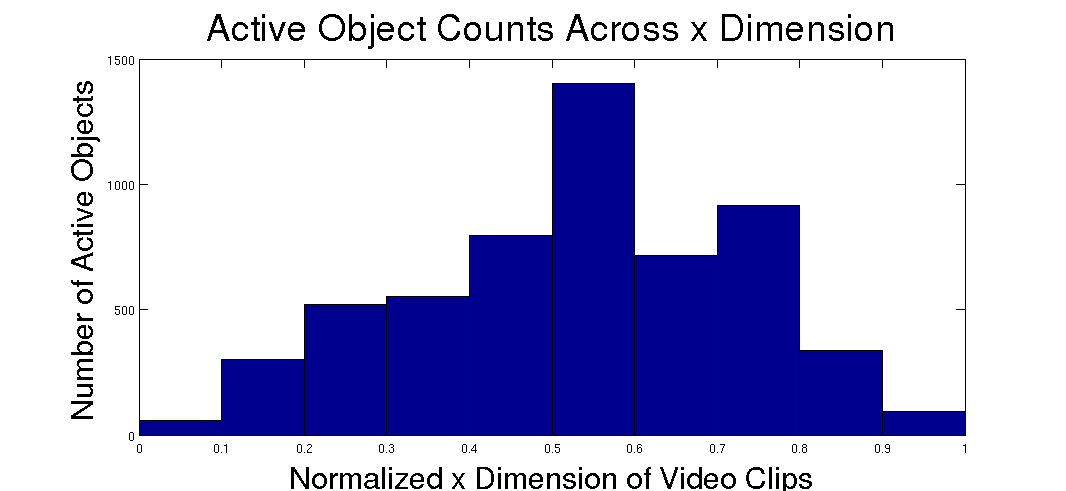
\includegraphics[width=5.9cm]{figures/active_obj_distr_x.png}}}&
\bmvaHangBox{\fbox{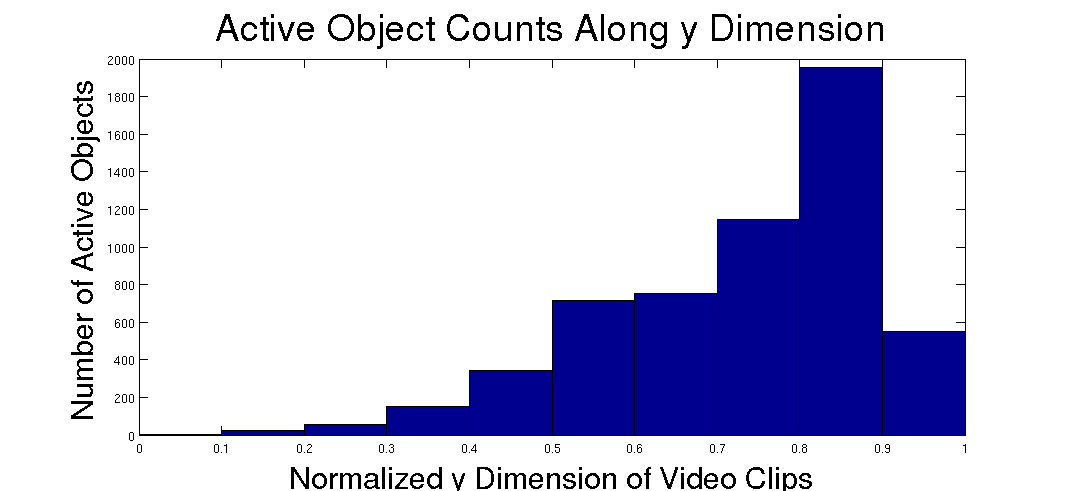
\includegraphics[width=5.9cm]{figures/active_obj_distr_y.png}}}\\
\end{tabular}
		   \caption{Histograms of detected active objects across the $x$ and
       $y$ spatial dimensions of training data. Active objects tend to appear in the lower
     center field of view. There is a slight bias favoring the
   right side of the field of view because many users are right-handed. }
\label{fig:teaser}
  \end{center}
\end{figure}
	
	From figure 2 we see that active objects often tend to occur in the lower center
	of the field of view. This conforms to our expectations, because
	the active objects are close to the hands which are in the lower field of
	view from an egocentric perspective. Active objects tend to occur on the
  right side of the field of view slightly more often because a large
  percentage of users are right-handed.
  The distribution of active objects
  across the temporal dimension is nearly uniform. 
  This distribution is computed across all action types; we do not compute
  separate active object distributions for each action class.
  Since different clips can have
  varying lengths with respect to time, we normalize the length of each
  video clip to 1 and consider relative temporal locations of active
  objects. 
	For biased partitions, we generate
  the first split along each dimension according to a distribution
  corresponding to the histograms of observed active object regions in the training data,
  and we generate all subsequent child cuts using a uniform distribution.
  For example, when generating a biased cut for the $y$ dimension, 
  we generate a random number between 0 and 1 that has a high probability of
  being in the range $(0.5, 0.9)$.
  We do not consider locations of passive objects at all during the
  generation of biased partition schemes.
  Since active objects are located
  in close spatial proximity to hands, creating object-centric partition schemes can
  be interpreted as implicitly taking into account information about hand
  locations.
	\begin{figure}[t]
		\begin{center}
			%\fbox{\rule{0pt}{2in} \rule{0.9\linewidth}{0pt}}
			  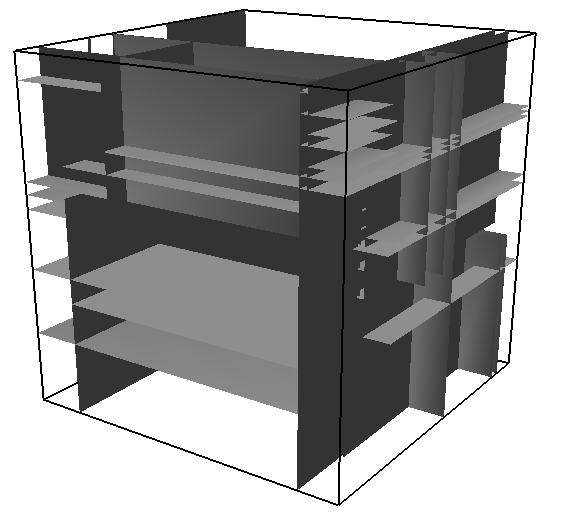
\includegraphics[width=6.0cm]{figures/lvl3-3.png}
		\end{center}
    \caption{An example 3-level object-centric partitioning scheme. Visible cuts along
    the $y$ dimension correspond to locations known to frequently contain
  active objects.} 
				\label{fig:long}
				\label{fig:onecol}
	\end{figure}
  
  Figure 3 depicts an example 3-level object-centric partition scheme. 
  The salient feature to note is that visible splits along the $y$
  dimension correspond to the observed distribution of active objects along
  the $y$ dimension of the training data.
  

\begin{figure}
  \begin{center}
\begin{tabular}{cc}
\bmvaHangBox{\fbox{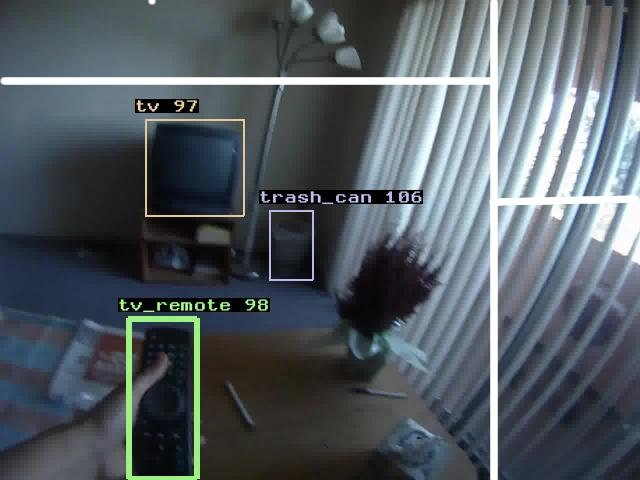
\includegraphics[width=5.9cm]{figures/unbiased_prt.jpg}}}&
\bmvaHangBox{\fbox{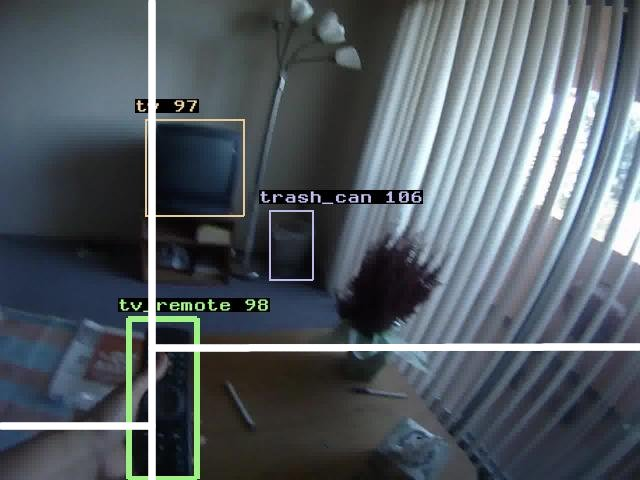
\includegraphics[width=5.9cm]{figures/biased_prt.jpg}}}\\
(a)&(b)\\
\end{tabular}
		   \caption{Potential partition schemes that could result using uniform
       (a) and object-centric (b) partition generation. The partition scheme
     resulting from using object-centric partition is likely to be more
   discriminative.}
\label{fig:teaser}
  \end{center}
\end{figure}
  
  \subsection{Complexity and Runtime}
  The asymptotic complexity of training with $N$ training examples 
  and a pool of $M$ candidate partition schemes with $l$ levels using our
  method is 
  \begin{center}
  $O(N\cdot M \cdot 8^l \cdot t_{train} + b \cdot (N + M \cdot t_{test}))$
  \end{center}
  where $b$ denotes the number of boosting rounds, and $t_{train}$ and
  $t_{test}$ denote the time to train and test a single SVM classifier on
  $N$ feature vectors, respectively. Fortunately, $l$ remains small (never
  exceeds 4 in our experiments). In order to predict the label for a single
  test video clip $v$, we first need to compute representations of $v$ using
  each partition scheme that was selected during boosting, then find the
  class $c$ which maximizes a weighted sum of matching classifications using
  each weak classifier selected during boosting.
  Thus, the overall
  asymptotic complexity of predicting the
  label for a single video clip is 
  \begin{center}
  $O(b \cdot 8^l + C \cdot b \cdot t)$
  \end{center}
  where $b$ is the number of boosting rounds, $C$ is the number of possible
  activity labels, and $t$ is the time to predict the label of a test
  example using a weak SVM classifier.
  
\begin{figure}
  \begin{center}
\bmvaHangBox{\fbox{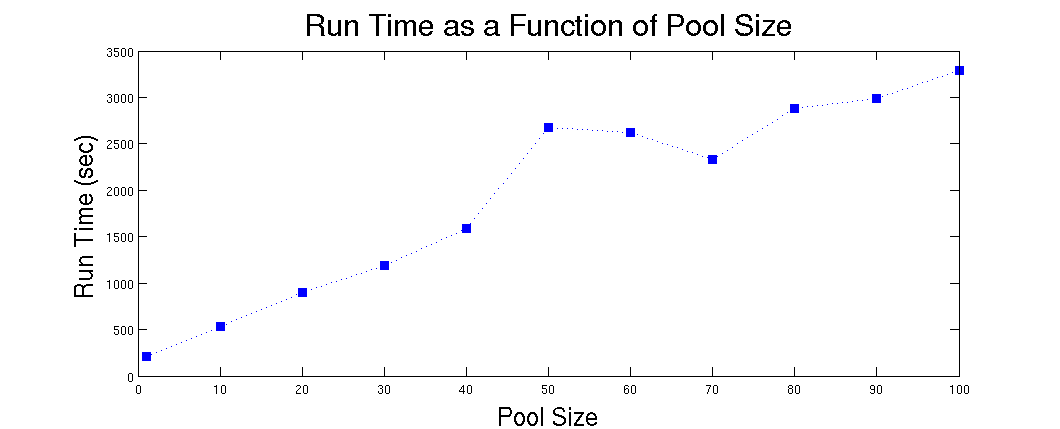
\includegraphics[width=9.0cm]{figures/runtime.png}}}\\
		   \caption{Running times for our method as a function of pool size.}
\label{fig:teaser}
  \end{center}
\end{figure}
  Figure 5 depicts empirically determined running times for our method on a
  single ``fold'' of the cross-validation experiment described in section
  3.1. For each pool size we present mean execution time across 5 separate
  executions. Running time is linear with respect to pool size.
  

\section{Results}
  In this section we briefly describe properties of the dataset we use to
  benchmark our method and present results from experiments we conducted. We
  evaluate our overall recognition accuracy and show that it improves the
  current state of the art, and we demonstrate the superior discriminative
  power of object-centric partition schemes.

  The ADL dataset consists of hundreds of egocentric video clips
	(roughly 10 hours of video in total) collected from 20 people performing
	18 types of unscripted actions in their own homes. These naturally
  occurring
  actions are often related to hygiene or food preparation and are more
  varied than actions presented in previous datasets such as that of \cite{Fathi11}.
  There are 26 different 
	types of detected objects, including 5 active and 21 passive objects. 
  Lists of activity types and object types are given in Table 1.
  Object detectors are trained on videos from the
  first 6 people and tested on the videos from the remaining 14 people.

\begin{table}
  \begin{center}
\begin{tabular}{cc}
\bmvaHangBox{\fbox{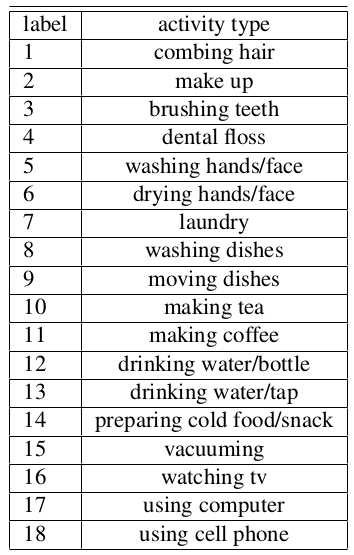
\includegraphics[width=4.0cm]{figures/actionlist.png}}}&
\bmvaHangBox{\fbox{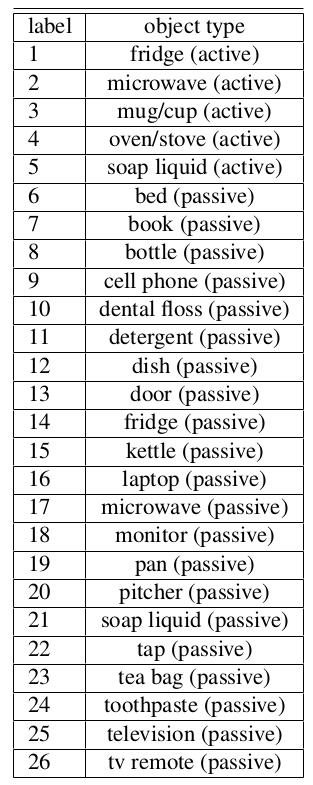
\includegraphics[width=4.0cm]{figures/objectlist.png}}}\\
\end{tabular}
		   \caption{Lists of action types and object types present in the
       ADL dataset. Separate active and passive models are trained for fridge,
     microwave, mug/cup, oven/stove, and soap liquid.}
\label{fig:teaser}
  \end{center}
 \end{table}
  

  
	Each frame in the dataset
	is annotated with activity labels and bounding boxes for detected objects and hand positions, 
	Additionally, each object is tagged as active or passive depending
	on whether it is being interacted with. 
  
  One difficulty that can arise within egocentric
  activity recognition is that activities can be temporarily interrupted by
  other activities. For instance, while waiting for tea to brew a subject
  may watch TV. For cases of such interruptions, to avoid unnecessary
  complications resulting from frames being annotated with multiple
  activities, the ADL dataset simply uses the label of the interrupting
  action when a longer action is disrupted.
  

	The ADL dataset has been modified since the publication of
	\cite{Ramanan12}; because of this, running the published code gives
	slightly lower accuracy than the originally published numbers. We use the
  modified version of the dataset available from the authors webpage at the time of writing to
  benchmark our method.   \subsection{Action Recognition Performance}
  Following \cite{Ramanan12}, we evaluate recognition performance on the ADL
  dataset using a form of cross
	validation (the video clips from person $i$ are used as a held out validation set, and
	training occurs using the video clips from the remaining people).
  We exclude videos from the first 6 people
  (because they were used to train the object detectors) from our
  experiments.

	  Table 2 shows a comparison of overall classification accuracy between our
  approach and the method based on temporal pyramids which is
  presented in \cite{Ramanan12}. The temporal pyramid
  has two levels, formed by making a single cut along the temporal
  dimension and no cuts along the spatial dimensions.
  These results were obtained
  using both active (being interacted with) and passive detected objects.
  The consideration of active objects when constructing feature vectors
  gives a significant improvement over just including passive objects.

  \begin{table}
		\begin{center}
			\begin{tabular}{|l|c|c|c|c|c|}
				\hline
        BoW & Temporal Pyramid \cite{Ramanan12} & RSTP & RSTP+OCC \\
				\hline\hline
        34.9\% & 36.9\% & 33.7\% & 38.7\%\\
				\hline
			\end{tabular}
		\end{center}
		\caption{Overall classification accuracy on pre-segmented video clips,
    evaluated using a form of cross validation. Our boosted RSTP+OCC classifier
  improves on the current state of the art.}
	\end{table}
  
	For this experiment we tried pools of 4-level partitioning schemes of
  varying sizes with a varying number of boosting rounds. The numbers
  presented in Table 2 were obtained with 5 boosting rounds and a pool of
  size 70.
  The work of \cite{Jiang12}, which uses a similar
  pyramid-based boosting approach for 2D image recognition, found that using
  pyramids with more than 3 levels actually led to a decrease in overall
  accuracy due to over-segmentation of image space. However, we found that in the
  3D case 4-level pyramids give better overall accuracy than coarser-grained
  representations.


  
  \begin{figure}
  \begin{center}
  \bmvaHangBox{\fbox{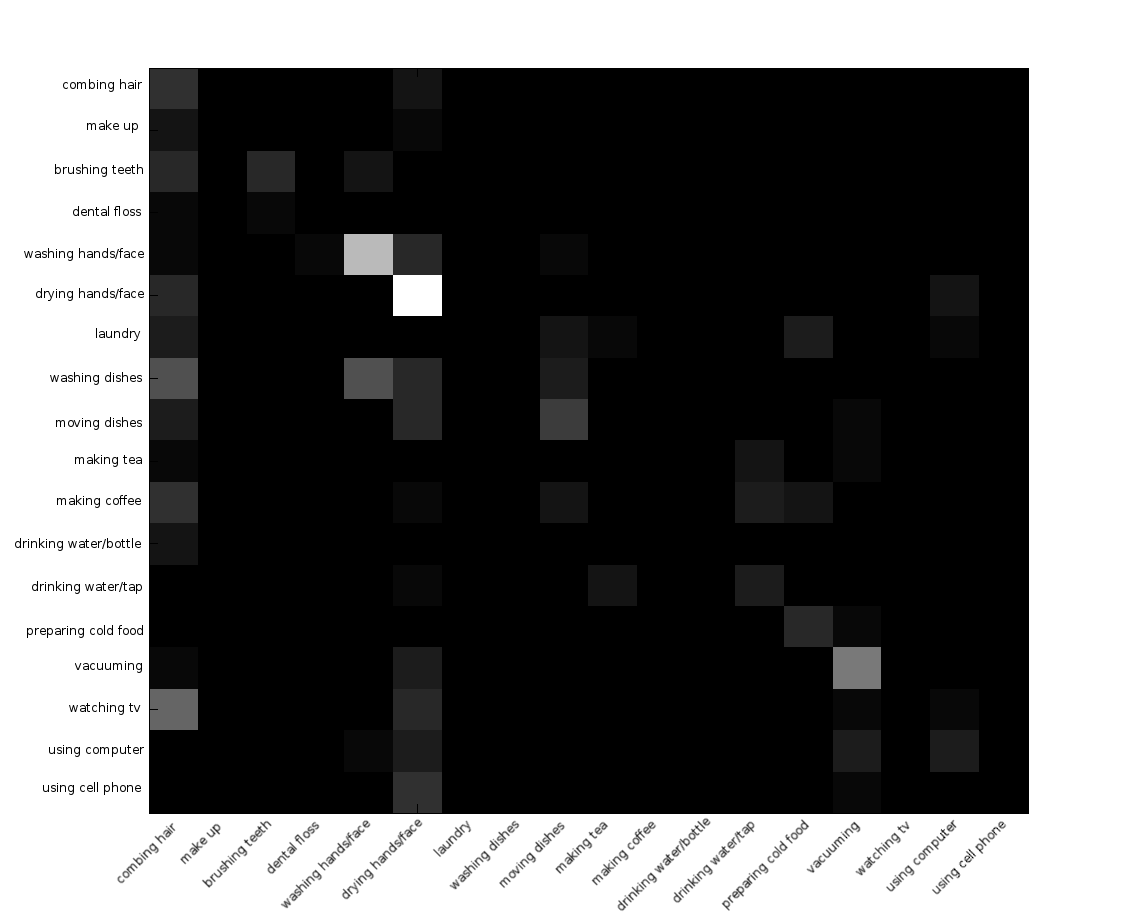
\includegraphics[width=10.0cm]{figures/confn2-labels.png}}}
		   \caption{Confusion matrix for RSTP+OCC using detected active and
       passive objects}
  \label{fig:teaser}
  \end{center}
  \end{figure}
 	As seen in Figure 6, our method has particularly good
  performance for activity types 5 and 6 (``combing hair'' and ``drying
  hands/face'', respectively). Some activity types on which our method does
  poorly are 10 and 11, which are ``making tea'' and ``making coffee'',
  respectively (see Table 1 for a full listing of activity types present in
  the ADL dataset). Since the two activity types are similar in the sense that
  they involve the same active objects, it is not
  unexpected that a recognition system would confuse them often.
  Furthermore, since the distributions of objects across space-time are
  similar, and kettles and tea bags are not modelled in an active way, it is
  difficult for our boosting algorithm to select partitioning schemes that
  are discriminative for these classes. An extension of our method which
  allowed selection of discriminative partition schemes on a per-class basis
  could allow for more fine-grained control and could help mitigate such
  issues.




  

  % training error exp
  \subsection{Effect of Object-Centric Partition Schemes}
  To concretely illustrate the improvement obtained from using a
  object-centric partitions, we created separate pools containing 4-level
  partition schemes of each bias type and
  repeatedly ran our boosting algorithm, computing training error and adding additional
  partitions to each pool between runs. Results from this experiment are
  depicted in Figure 7. The pool containing object-centric partitions 
  usually had a lower training error than the unbiased pool.
  Larger improvements are visible with smaller pool sizes, and the difference
  between the two pools diminishes as pool size increases. This conforms to
  expectations because as the unbiased pool grows in size, it becomes more
  likely to contain discriminative partition schemes, while the biased pool
  is forced to contain discriminative partition schemes even at relatively
  small pool sizes. This result suggests that by using object-centric
  partitions rather than unbiased partitions, we can obtain good recognition
  results even with a smaller pool, making our boosting algorithm less expensive
  to compute.
 
  \begin{figure}[t]
		\begin{center}
			%\fbox{\rule{0pt}{2in} \rule{0.9\linewidth}{0pt}}
			  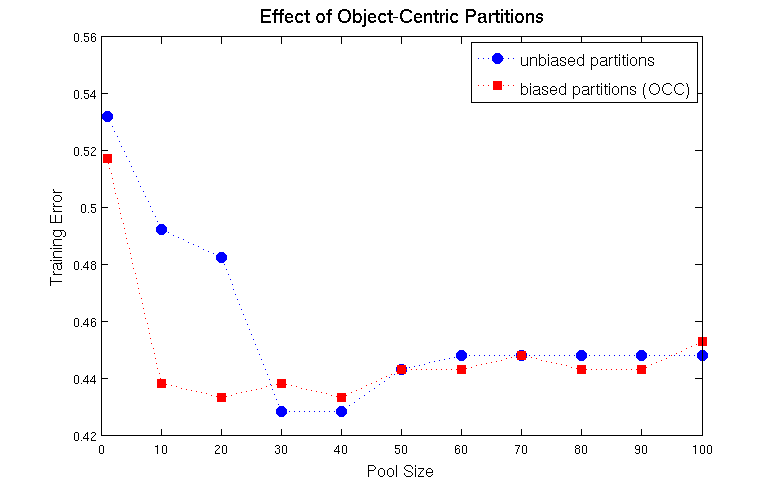
\includegraphics[width=1.0\linewidth]{figures/trainerror.png}
		\end{center}
		   \caption{Effect of using biased partition schemes. The object-centric
         pool
       usually has lower training error
       than the pool of unbiased partition schemes. The most significant
     improvement is visible at smaller pool sizes.}
				\label{fig:long}
				\label{fig:onecol}
	\end{figure}
  
	
\section{Conclusion and Future Work}
	Our main novel contribution is two-fold. We show how to learn the most
  discriminative partition schemes for spatio-temporal binning in video feature space, and
  we introduce object-centric partition schemes, which have a high
  probability of cutting through video regions known to frequently contain
  active objects. Unlike previous work, we randomly generate a pool of
  candidate partitioning schemes and select those which are most
  discriminative using a boosting algorithm.
  Our recognition approach improves on the current state of the art, and our
  experiments demonstrate the positive impact of taking active object
  locations into account by generating object-centric partition schemes.
  
  In future work, we intend to investigate ways of learning the most
  discriminative partition schemes on a per-class basis.
	Additionally, it may be possible to incorporate different types of biases when generating
	partitions. The ADL dataset also includes annotations for hand positions,
	which we have incorporated implicitly through our generation of
  object-centric cuts.
	However,
	it could be possible to incorporate explicit information given by hand
	positions to obtain better results.
	The partitions we focus on contain cuts that are
  planar and axis-aligned (we consider random shifts but not random
  rotations, and we do not consider non-planar splits),
  but it is possible to carve up the
	video volume in more advanced non-linear ways. Such a method would 
  make histogram computation more expensive	, but may yield a more discriminative
	partitioning scheme that could lead to better classification accuracy.
\bibliography{egbib}
\end{document}
